\documentclass[
a4paper, 
%a5paper,
%10pt,
%11pt,
12pt,
%twoside, % single sided printout
%oneside, % duplex printout (default)
%% binding correction is used to compensate for the paper lost during binding
%% of the document
%BCOR=0.7cm, % binding correction
%nobcorignoretitle, % do not ignore BCOR for title page
%% the following two options only concern the graphics included by the document
%% class
%grayscaletitle, % keep the title in grayscale
grayscalebody, % keep the rest of the document in grayscale
abstract=on,
%% expert options: your mileage may vary
%baseclass=scrreprt % special option to use a different document baseclass
twoside, BCOR10mm, 12pt, DIV13,headinclude, footexclude, final, abstracton, openright
]{ibireprt}


\usepackage[utf8]{inputenc}
%\usepackage[latin1]{inputenc}
\usepackage[T1]{fontenc}
%\usepackage{ngerman}
\usepackage[ngerman]{babel} %english,


%\usepackage{fancyhdr}
%%\pagestyle{fancy}
%%\lhead{\leftmark}
%\fancyhead[OR]{\thepage}% ungerade Seiten, rechts \thepage
%\fancyhead[OL]{\leftmark}% ungerade Seiten, links
%\fancyhead[ER]{\leftmark}% gerade Seiten, rechts
%\fancyhead[EL]{\thepage}% gerade Seiten, links \thepage
%\cfoot{}
%\pagestyle{fancy}

\renewcommand{\chaptermark}[1]{\markboth{#1}{}}
\renewcommand{\sectionmark}[1]{\markright{#1}{}}

\setlength{\parindent}{0em}
%\setlength{\parskip}{0mm}
\setcounter{tocdepth}{1}
\setcounter{secnumdepth}{2}
%\linespread{1.15}

\usepackage{quotchap}
\usepackage{nccmath}

\usepackage{microtype}

\usepackage{qtxmath,tgtermes}
\usepackage[scaled=.90]{helvet}
\usepackage{courier}

\usepackage{graphicx}
\usepackage{amsmath}
%\usepackage{amsfonts}
\usepackage{amssymb}
\usepackage{tabularx}
%\usepackage[bookmarks,plainpages=false]{hyperref} %colorlinks  ,urlbordercolor={111},linkbordercolor={111},citebordercolor={111}
\usepackage[Algorithmus]{algorithm}
\usepackage{algorithmic}
%\usepackage{tkmath}
\usepackage{exscale}
\usepackage{empheq}
\usepackage{color}
\usepackage{framed}
\usepackage{rotating}
\usepackage{longtable}
\usepackage[hang,small,bf]{caption}
\usepackage{booktabs}
\usepackage{colortbl}

\usepackage[babel,german=quotes]{csquotes}
\usepackage{ntheorem}
\usepackage{blindtext}

%\mathindent1.5cm
\def\fleq{\@fleqntrue \let\mathindent\@mathmargin \@mathmargin=\leftmargini}
\def\cneq{\@fleqnfalse}


%\setcapindent{0em}

\newenvironment{fshaded}{%
\def\FrameCommand{\fcolorbox{framecolor}{shadecolor}}%
\MakeFramed {\FrameRestore}}%
{\endMakeFramed}

\theoremseparator{:}

\newtheorem{theorem}{Theorem}[chapter]
\newtheorem{lemma}{Lemma}[chapter]
\newtheorem{remark}[theorem]{Bemerkung}
\newtheorem{definition}[theorem]{Definition}
\newtheorem{example}{Beispiel}
%\newtheorem{proof}[theorem]{Beweis}
\newtheorem{corollary}[theorem]{Corollary}

\newenvironment{Theorem}{\goodbreak \definecolor{shadecolor}{rgb}{0.95,0.95,0.95}%
\definecolor{framecolor}{rgb}{0,0,0}%
\begin{fshaded}\begin{theorem}\sl}{\end{theorem} \end{fshaded}}
\newenvironment{Lemma}{\goodbreak \definecolor{shadecolor}{rgb}{0.95,0.95,0.95}%
\definecolor{framecolor}{rgb}{0,0,0}%
\begin{fshaded} \begin{lemma}\sl}{\end{lemma} \end{fshaded}}
\newenvironment{Remark}{\goodbreak \begin{remark}\rm}{\hfill  $\square$\end{remark}}
\newenvironment{Example}{\goodbreak \begin{example}\rm}{\hfill $\square$ \end{example}}
%\newenvironment{Proof}{\goodbreak \begin{proof}\rm}{\hfill $\blacksquare$ \end{proof}}
\newenvironment{Definition}{\goodbreak \definecolor{shadecolor}{rgb}{0.95,0.95,0.95}%
\definecolor{framecolor}{rgb}{0,0,0}%
\begin{fshaded} \begin{definition}\rm}{\hfill  \end{definition} \end{fshaded} }
\newenvironment{Corollary}{\goodbreak \begin{corollary}\rm}{\end{corollary}}

\newenvironment{Proof}[1][Beweis:]{\begin{trivlist}
\item[\hskip \labelsep {\bfseries #1}]}{\hfill $\blacksquare$\end{trivlist}}

\numberwithin{equation}{chapter}
\numberwithin{table}{chapter}
\numberwithin{figure}{chapter}
\numberwithin{algorithm}{chapter}
\numberwithin{example}{chapter}
\numberwithin{example}{chapter}

\def\i{\mbox{\small{\rm i}}}
\def\ti{\mbox{\scriptsize{\rm i}}}
\newcommand{\e}[1]{{\rm e}^{ #1}}
\renewcommand{\mod}{\;{\rm mod}\;}

\newcommand{\zb}[1]{\mbox{\boldmath{${#1}$}}}
\newcommand{\zbs}[1]{\mbox{\boldmath\scriptsize{${#1}$}}}
\newcommand{\zbss}[1]{\mbox{\boldmath\tiny{${#1}$}}}

\newcommand{\adj}{{\ensuremath{\mathsf{H}}}}
\newcommand{\trans}{{\ensuremath{\mathsf{T}}}}


% Keine "Schusterjungen"
\clubpenalty = 10000
% Keine "Hurenkinder"
\widowpenalty = 10000 \displaywidowpenalty = 10000 %\displaywidowpenalty = 10000






% Information for the Titlepage
\author{Johann Strunck}
\title{Deep learning based grading of motionartifacts in HR-pQCT}
%\date{\today}
\date{\today}
\subject{Bachelor thesis}
\professor{Prof.~Dr.-Ing.~Tobias Knopp}
\advisor{Dr.~rer.~nat.~Martin Hofmann}







\begin{document}
%\frontmatter
\maketitle
%\mainmatter


\newpage
${}^{}$
\vfill
\noindent
Ich versichere an Eides statt, die vorliegende Arbeit selbstständig und nur unter Benutzung der angegebenen Quellen und Hilfsmittel angefertigt zu haben.\\
\vspace{1.5cm}

\noindent
Hamburg, den ??.??.2010
\thispagestyle{empty}
\newpage
\newpage

\setlength{\parskip}{1.5mm }

%\newpage

%\maketitle



\tableofcontents


\chapter*{Summary}
	A common issue of High-resolution peripheral quantitative computed tomography (HR-pQCT) scans is the appearance of motion artifacts in Images. These artifacts can appear due to involuntary movements like twitches and spasms. Since a scan can last between 3-4 minutes its hard not to move for such a long time. Depending on the severeness of those artifacts in the resulting image, it might not be sufficient for medical use and a re scan is necessary. The decision of the severity is decided by a professional which gives the image a number from 1 to 5, where 1 equals no motion artifacts and 5 equals severe motion artifacts. The descission of severity can be biased and varies depending on the reviewing person. Studies showed that operators disagree in up to 30\% of all cases.
	 To support the descission of the operation there have been approaches by \cite{Sode2011} and \cite{Walle2023}  to improve the confidence of the result. both methodes can be performed with the absence of a operator and results of \cite{Sode2011} show that with crossvalidation of a operator  a Convolutional Neural Network(CNN) can reach a higher accuracy than the cross validation of two operators without a CNN. The CNN still has a considerable error rate. In this paper we will propose a new CNN structure which uses state of the art methods to detect the severity of motion Scores in CT scans. 

\chapter{Introduction}

High-resolution peripheral quantitative computed tomography (HR-pQCT) is a specialized non-invasive imaging technique that provides detailed and accurate three-dimensional images of bone and tissue microarchitecture at the peripheral skeletal sites. In our paper we focus  on the radius and thibia. This advanced imaging modality offers several distinct advantages. One advantage is that HR-pQCT provides high resolution images that allow a thorough assessment of a scanned bone micro architecture. It offers precise measurement of bone mineral density(BMD) and geometric parameters such as trabecular thickness and cortical thickness. HR-pQCT has applications in both clinical and research setting and can help make more informed decissions about patient management and treatment strategies. It can provide insight into fracture or the risk of its occurrence. HR-pQCT imaging requires the patient to remain still during the scan to avoid motion artifacts. This can be challenging for certain patient populations, such as children or individuals with limited  mobility. Especially with the XtremCT (Scanco Media AG),a device that  was used to generated the test and training data for this paper.The XtremCT takes about 3-4 Minutes for a scan which makes it hard to hold the chosen extremity in place for such a long time.

 Depending on the severity of the motion artifact the scan must be repeated. To determine the severity of the scan \cite{Whittier2020} Introduced a scale from 1 (no visible motion artefacts) to 5 (significant horizontal streaks). In clinical studies it is commonly implemented, that scans with a grading of 4 or 5 have to be repeated to mitigate the effects of the motion artifacts. However, even with a standardized scoring system, motion scoring remains subjective, and operator agreement has shown to remain only moderate, even with intensive training [], studies have shown that operators disagree in up to 30\% of all cases[look at bone]. Due to this issue a objective and standardized method is desirable for the grading process. Papers like \cite{Sode2011} and \cite{Walle2023} have taken an approach to find a suitable methode for grading motion artifacts, with partial success.
 
\cite{Walle2023} proposes a method for objective detection of subject motion. The first method measures subject motion by comparing the projections at 0° and 180° since those projections are parallelized, the should be the mirror of each other when no subject motion occurred. Therefore by comparing the difference of those two parallel projections the subject motion can be approximated. This method is called Quantitative Motion Estimate and utilizes a similarity measure like the sum of squared intensity difference(SSD) or normalized cross correlation (NCC) to compare the mirrored parallel projection image at 0° and 180°.

In resent years a tremendous intrest in deep learning networks has emerged \cite{LeCun2015} ...\cite{Yamashita2018} %TODO: look at this paper to write this part another paper is
 %vlt zu konkret das sollte glaube ich eher in die beschreibung der algorithmen rein kommen 
  %The main Constrain of this approach is that the subject could move and then land in the same position which would lead to a wrong label.
 
  

\cite{Sode2011} uses the power of CNNs to train a network for grading motion artifacts. Deep learning techniques, particularly CNNs, have revolutionized medical image analysis. CNNs are a %TODO: short description of cnns maybe also about the use of medical imaging in other arreas 
CNNs excel at tasks such as image segmentation, object detection, and classification. With their ability to automatically learn intricate patterns and features from complex visual data, enabling more accurate and efficient diagnostic processes. %more information necessary 
Even with the simplistic structure chosen in \cite{Sode2011} the Network is reaching a accuracy of ..., this can lead to the assumtion that a more suffisticated network might be more suitable . In this paper we will build on those findings and try to create a stronger network with state of the art CNN building blocks 


%TODO: part about CNN's
In this paper we will introduce a Convolutional Neural Network Structure which is designed to predict the severity of the motion artifact and compare this Structure to the findings of \cite{Sode2011} and \cite{Walle2023}. 

The data that we use in this paper to compare the different approaches was provided by the "Universitäts Klinikum Eppendorf". All 500 provided scans where generated by the Scanco XtremCT.% maybe explain the basics of ct scans 
to ensure the correctness of the labeled data three doctors of the institution labeled the data together to ensure that the data was generalized and reduce the subjective influence of the single person  


A frequently occurring issue in medical imaging is the lack of training data. In our case we had 500 labeled examples of tibia and radius. If we compare this to the amount of data used in training state of the art networks like ImageNet with many Million Examples it's a small fraction. This comes on the one hand from the fact that the labeling task in medical imaging can just be performed my professionals and therefore the labeling process is costly and just a few people can do it. Another issue is the availability of data since patient data cant be accessed and used as easy. Therefore we need to find a way to augment the data so that we don't run into problems like overfitting the Network or poor generalization of the network
\chapter{Literature review}

\begin{figure}[h]	
	\center
	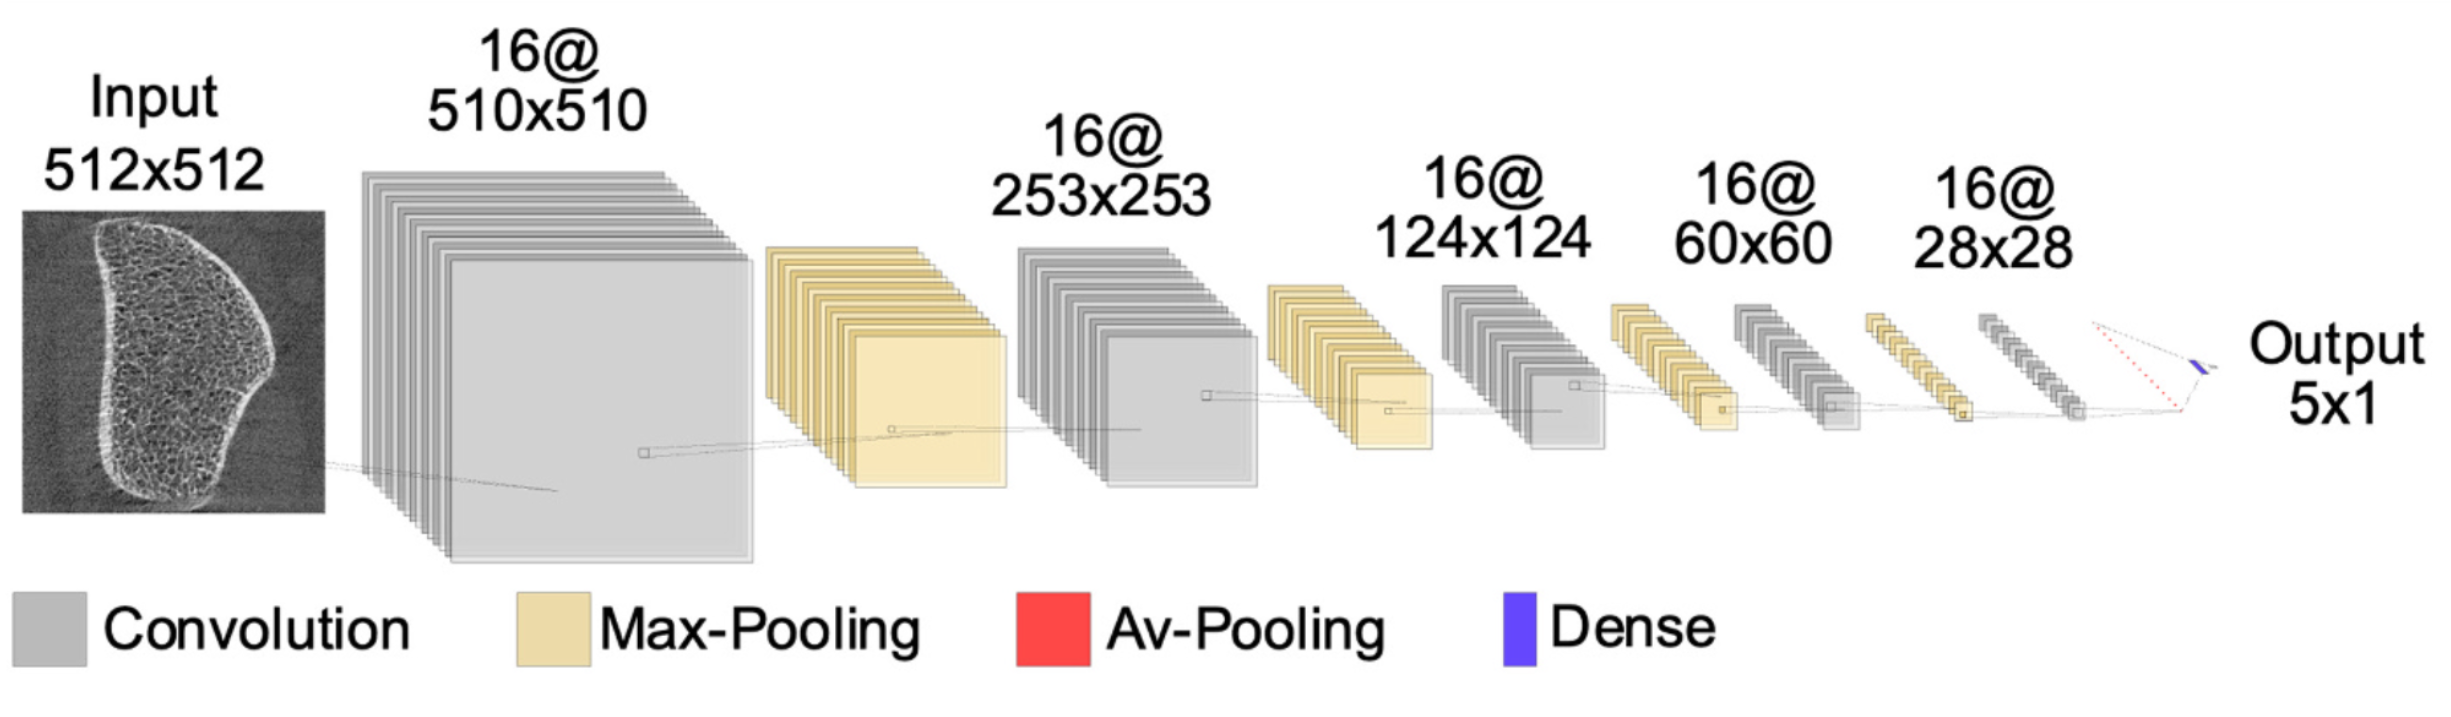
\includegraphics[width = 1 \textwidth]{Bone_Network_Structure.png}%
	\caption{Network Structure Bone}
	\label{fig:fig1}
\end{figure}%

Bone et al introduces a CNN in his paper which he trained to classify the severity of motion artifacts in HR-pQCT. He trained his network with images(XtremeCT II, Scanco Media AG) from 90 patients. The size of the scans was 512 x 512 x 168. for the training he used 8 equally spaced images from every scan  resulting in a database of 3312 images.
The implemented Network strucuture begins with five alternating convolutional and max-pooling layers followed by a average pooling layer and is concluded by a dense layer. To extract the most important features max Pooling was used followed by a convolutional layer to aggregate them. Convolutional layer used (LeakyReLu) activation to enable faster learning while avoiding dead neurons.
%aufpassen einfach koppiert vlt umformulieren 
 The classification was performed by a Fully Connected layer r integrating non-linear combinations of all high-level features using a standard Rectified Linear
Unit (ReLU) activation function . On the output layer, a Softmax activation function provided an output that may be understood as a class probability, with each output larger than zero and their total always equal to one

\chapter{Methods}
%CT
Computer tomography(CT) uses a three dimensional radiographic imaging technique. The formation process begins with the acquisition of sequential radiographic projections captured over a range of angular positions around the object of interest. The crossectional field of view is reconstructed using established computational techniques based on the radon projection theory\cite{article}.Similar to simple radiography, the reconstructed image’s intensity values represent the local radiographic attenuation: a material property related to the object’s electron density (atomic number and mass density). The contrast between soft and mineralized tissue in CT is high, due to the relative electron-dense inorganic component (calcium hydroxyapatite) of the bone matrix.These principles capture high-resolution images of bone
across a range of structural scales. %das habe ich koppiert (muss unbedingt umgeschrieben werden )
%HR-pQCT
High resolution peripheral quantitative computer tomography(HR-pQCT) is a  dedicated extremity imaging system designed for trabecular-scale imaging and is currently available from a single manufacturer (XtremeCT; Scanco Medical AG,
Bru¨ttisellen, Switzerland). 


%CNN
Convolutional Neural Networks (CNNs) are a class of deep learning models specifically designed for processing structured grid-like data, such as images, by automatically learning hierarchical patterns and features. CNNs are widely used in computer vision tasks and have revolutionized the field of image recognition, object detection, and image generation. CNNs excel at tasks like image classification, where the network assigns a label or category to an input image\\
%Convolutional Layer
The fundamental building blocks of CNNs are convolutional layers, which perform convolution operations on input data. These layers apply a set of learnable filters (also called kernels) to input images by sliding the filter over the input data and computing element-wise multiplications and summations to produce feature maps. This layers purpose is detecting different features like edges, textures, and more complex patterns. The learned features become progressively more abstract as they pass through multiple convolutional layers making it possible to classify complex structures.	Two key hyperparameters that define the convolution operation are size and number of kernels. The former is typically 3 × 3, but sometimes 5 × 5 or 7 × 7. The application of a Convolutional layer on a Matrix, shrinks it in size, to mitigate this effect there are two other parameters that can be set to get the desirable output size. On the one hand we kann add Padding, this adds number rows and columns of zeros to the matrix to increase the output size. During the convolution,the filter slides over the matrix from left to right and top to bottom, stride is defined as the step size of the filter, meaning its the definition of how many elements the filter moves to the right or bottom.\\
%Pooling Layer
The Convolutional layer is usually followed by a Pooling layer. This  layers downsample the feature maps, reducing the spatial dimensions while retaining important information.Usually The stride matches the filed size of the pooling operation, so that no feature of the previous layer is used twice. Max pooling and average pooling are the most common applied pooling operations. In the Max pooling opperation the maximum value of the current view is selected, this preserves detected features especially the most commonly used ones. The average pooling operation takes the averages of the values of the current view. During training in back propagation average pooling provides a smoother gradient compared to max pooling. It also retains information from the original image since average pooling takes the collective information into account. \\ 
%TODO: Bring more mathematical expressions in the mix
%Fully Connected Layer
The fully connected layer connects all neurons from the previous layer to all neurons in the subsequent layer, enabling the network to make high-level decisions based on the learned features. The neurons of this layer are organized in a array form. This layer is used to optimize objectives as class scores.\\
%Data Augmentation
A big issue in the space of medical imaging is the lack of training data. When training a CNN with to little data we either have to stop early and don't get a optimal accuracy for the network. If we would further train the network with the same samples the network would overfit and lose its validity  
therefore we nee to find a way to augment the data so that it still has the same meaning for a person. The concept of data augmentation is well spread in the medical imaging field 
to use data augmentaiton techniques like rotation 

\begin{align}
 \zb S &= \zb c \zb u
\end{align}

\chapter{Experimental Setup}



\chapter{Results}

\chapter{Discussion}

\bibliographystyle{unsrt} %unsrt abbrv
\bibliography{Bibliography}

\end{document}
